\documentclass[a4paper, 11pt]{article}
\usepackage{multicol} % Multi columns
\usepackage{comment} % enables the use of multi-line comments (\ifx \fi) 
\usepackage{lipsum} %This package just generates Lorem Ipsum filler text. 
\usepackage{fullpage} % changes the margin
\PassOptionsToPackage{hyphens}{url}\usepackage{hyperref} % Links
\usepackage[inline, shortlabels]{enumitem} % Inline item lists
\usepackage{mathtools} % Math
\usepackage[toc,page]{appendix} % Appendix
\usepackage{graphicx} % For images
\usepackage{pdfpages} % Full page images
\usepackage{subcaption}
\usepackage{fancyref} % Referencing images
\usepackage{lineno}
\usepackage[compact]{titlesec} % More compact layout
\usepackage{caption}

\begin{document}
%Header-Make sure you update this information!!!!
\noindent
\large\textbf{OpenMP project - Design Document} \hfill \textbf{DEBS 2013 - Soccer Monitoring} \\
\normalsize Middleware Technologies \hfill Arcari Leonardo \\
Prof. Mottola \hfill Cilloni Stefano \\
A.Y. 2017 - 2018 \hfill Gregori Giacomo
\noindent\rule{\columnwidth}{0.4pt}

\begin{multicols}{2}
\section{Introduction}
\subsection{Scope}
This document provides a description of the design of our solution to the DEBS 2013 Grand Challenge \cite{DEBS} in its simplified version \cite{Project}.

\subsection{Definitions, abbreviations}
\paragraph{$\mathbf{T}$} Number of seconds every which to output partial statistics.
\paragraph{$\mathbf{K}$} Maximum distance (in meters) a player is eligible for ball possession.
\paragraph{\textbf{Critical section}} A section of a program that can be executed only by one thread at a time. In some languages this is called a \texttt{synchronized} section.

\subsection{Assumptions}
Together with the assumptions already set in \cite{Project}, we set others taking them from the FAQ section of \cite{DEBS}.
\begin{enumerate*}[(a)]
    \item The playing field is approximated as a perfect rectangle whose vertices are at the following coordinates: $(0, 33965)$, $(0, -33960)$, $(52483, 33965)$, $(52483, -33960)$.
    \item Each player has at least 2 sensors. His position is computed as the average of the positions of his sensors.
    \item Towards the end of the first half they had a problem with ball transmitters, so computing the ball position is meaningless within that time interval. Therefore we set the end of the first half of the match to the time instant this problem arises, cutting out the last $2.5$ seconds.
\end{enumerate*}

\section{Technologies}
Our solution to the problem adopts C++ as programming language (standard 2017). The choice was justified by the language \emph{zero-cost abstraction} philosophy that allowed us to structure the code according to good OO design principles without sacrificing performance. Moreover we used OpenMP \cite{omp} as parallelization paradigm because it made it possible to design the application workflow sequentially and easily introduce parallelism in those sections that could benefit.

\section{Architectural Design}
In this section we describe our application architecture along with a rationale of the design choices. We start from a few numerical considerations. The application is required to be a \textit{real-time stream processor} of data arriving at a frequency of $2000Hz$ for ball position events and $200Hz$ for players position events, summing up to roughly $15000$ events per second. For the purpose of computing the ball possession, given a single upcoming player position event only one \textit{ball-player} distance is required to decide which player is the closest, because the distance of the ball from all the other players is left unchanged. Although, for a ball position event we must compute the distance for all the players with the new position of the ball to elect the ball possessor, keeping in mind that the ball position update frequency is $10$ times the players' one. Therefore we opted for a solution that could exploit as much as possible the available parallelism in the process.

The application architecture is composed of the following main components:
\begin{enumerate*}[(a)]
    \item \texttt{EventFetcher} reads the incoming events sequentially from the dataset, parses them and adds them to a \textit{mini-batch} of variable size.
    \item \texttt{GameStatistics} receives a mini-batch and it elects the ball possessor \emph{per time-instant}. It accumulates the number of times a player was in possession of the ball and outputs partial and whole-game statistics.
    \item \texttt{Visualizer} gracefully displays the computed statistics on the desired output stream.
\end{enumerate*}

A UML sequence diagram of the components interaction is reported in Figure~\ref{fig:top_level_seq}.

\section{Algorithms Design}
\subsection{Events parsing}
The process of events parsing hides two choices that are worth mentioning. As the position updates arrive as a stream we must keep a stateful \texttt{context} registering current position of each sensor on the field. It is \texttt{EventFetcher} responsibility to update it as long as new events arrive. Moreover, events meaningful for ball possession statistics are grouped in \texttt{mini-batches}. The decision of employing mini-batches was taken to maximize the parallelization impact on the application performance. In fact, moving a large number of events to the processors caches considerably reduces the application time spent in I/O operations, since the number of \textit{reads} from secondary memory becomes less than the number of events. When a batch is either full, the game is paused or $\mathbf{T}$ seconds of game are elapsed, the batch is sent to \texttt{GameStatistics}.

\subsection{Accumulating ball possessions}
\label{sec:accumul}
This is the parallel section of our application. We want to compute the ball possessor at each time instant. How do we discretize the time? We know that player sensors events arrive at a frequency of $200Hz$ while ball sensors transmit at a frequency of $2000Hz$. This order of magnitude of difference convinced us to use ball position updates as \textit{time-instants}. The process to compute ball possessions is reported in the sequence diagram in Figure~\ref{fig:accumulate_stats_seq} and hereby described.

First, we instantiate a \texttt{shared} structure $\mathcal{B}$ to store the ball possessor for each time instant. Then for each player \texttt{p} on the field we perform the following \textbf{in parallel}:
\begin{enumerate*}[(a)]
    \item Store a structure $\mathcal{D}$ to hold a list of \textit{ball-player} distances.
    \item Store a local copy of player \texttt{p} and ball positions at the time instant the first event was added to the mini-batch.
    \item For each event in the batch do the following: if it is an update on the position of player \texttt{p} then update the local copy of \texttt{p} position. If instead it is a ball position event, first update the local ball position, then compute the distance $d$ between the local position of \texttt{p} and the new position of the ball. If $d \leq \mathbf{K}$ then append $d$ to $\mathcal{D}$. Otherwise append $\infty$.
    \item After going through all the events, \textit{reduce} $\mathcal{D}$ to $\mathcal{B}$ in a \texttt{critical} section. That is, if $\mathcal{B}$ is empty, just copy $\mathcal{D}$ to $\mathcal{B}$. Otherwise, for each time instant $t$ check if $\mathcal{D}_t < \mathcal{B}_t$. If so, store in $\mathcal{B}_t$ that \texttt{p} is the current closest player, together with its distance $\mathcal{D}_t$. Because the number of ball position events is seen equal by all the threads, we are sure that $\mathcal{B}$ and $\mathcal{D}$ dimensions are the same across all the threads.
    \item When all the threads are done, go through all the elements $(min\_distance, p')$ of $\mathcal{B}$ and increment the ball possession count for player $p'$ by $1$ if $min\_distance \neq \infty$.
\end{enumerate*}

\subsection{Computing partial statistics}
In section~\ref{sec:accumul} we described how we compute the number of times a player is in ball possession. Computing partial statistics from that is straightforward. When $\mathbf{T}$ seconds of game are elapsed, a \textit{weighted-average} of the players possessions is performed. Let $\mathcal{A}$ be the accumulator, such that $\mathcal{A}_p$ is the number of instants the player $p$ was in possession of the ball. Let $total = \sum_p \mathcal{A}_p$. Then the partial ball possession statistics for player $p$ is $\mathcal{A}_p / total$. After computing partials, the accumulator is summed to the \emph{whole-game-accumulator} for final game statistics and then it is erased to accumulate the next $\mathbf{T}$ seconds of events.

\section{Implementation details}
\subsection{Data preparation}
As it was provided, the dataset contained different files for the sensors position events and the game interruption events. To make the stream processing possible we merged, through a preprocessing phase, the two files of game interrupts and game events into a single one. 
\subsection{Managing multiple balls}
As reported in the metadata, there are 4 balls each one with its sensor that transmit their position. In order to decide the ball we should compute the distance from we abstracted this away by means of a single \texttt{BallPosition} class. This class stores all the 4 sensors, but exposes only the position of the \textit{in-game} ball, that is the ball currently within the field rectangle. Whenever a sensor is registered as inside the field rectangle, that becomes the position of the \textit{in-game} ball. When the \textit{in-game} ball goes out of the field, \texttt{BallPosition} returns an infinite-distant position for the ball. This way, every distance computed with respect to the ball results in an infinite distance and does not participate in the ball possession statistics.

\section{Timing analysis}
In this section we report the timing analysis of our application to show that the \textit{real-time} requirement is satisfied. We ran the experiments on a Macbook Pro Mid-2012 shipping a Intel(R) Core(TM) i7-3615QM CPU @ 2.30GHz (4 cores, 2 threads per core). All the experiments are run with $\mathbf{K} = 5 m$ which maximizes the number of players eligible for ball possession. Results are reported in Table~\ref{tab:timings}. From our results we can conclude that the \textit{real-time} constraint is satisfied as we are able to process 1 second of events in less than 1 clock second. Specifically, we are able to satisfy this constraint in half of the time if we set the batch size to 1 (i.e. every event is processed right away) and in $1 / 30th$ of the time if we set the batch size to $10^7$ and we are asked to output partials every 60 seconds.

%-----------------------------------------------------------------------------
% Timing table - 1
%-----------------------------------------------------------------------------
\begin{center}
\begin{tabular}{|p{.15\columnwidth}|p{.15\columnwidth}|p{.2\columnwidth}|p{.25\columnwidth}|}
\hline
$\mathbf{T}$ (s) & Batch size & Resp. time (s) & Resp. time per sec\\
\hline\hline
$1$ & $1$ & $0.28$ & $0.28$\\
$1$ & $10^7$ & $0.05$ & $0.05$\\
$60$ & $1$ & $16$ & $0.27$\\
$60$ & $10^7$ & $1.8$ & $\mathbf{0.03}$\\
\hline
\end{tabular}
\captionsetup{width=0.9\linewidth}
\captionof{table}{Application response time [$n_{threads} = 4$]}
\label{tab:timings}
\end{center}
%-----------------------------------------------------------------------------

\section{Parallelization factor}
In this section we report the effectiveness of our parallelization strategy. We ran an experiment to jointly explore the average response time w.r.t. the number of threads and the batch size \cite{speedup}. In Figure~\ref{fig:perf1} we plot the response time and the speedup w.r.t. the single thread execution. In this experiments we discovered that the best combination for our machine was $n_{threads} = 4$ and $BatchSize = 10^7$. Projecting the analysis on the $BatchSize = 10^7$ axis we illustrate the impact of the number of threads on the execution time, as shown in Figure~\ref{fig:perf2}. We achieved a speedup of $27\%$ w.r.t. the single-thread execution running on 4 threads. The performance decrease with 8 threads was predictable. By enabling \texttt{-O3} optimizations the compiler will most likely introduce vectorial instructions in the application binary and in general there is a single vectorial ALU on each processor, making the \textit{hyper-threading} penalizing.

\section{Code analysis}
The application code was analyzed with Valgrind \cite{valgrind} to check for any memory access error which it resulted free of. Moreover the code was constantly profiled with Linux Perf \cite{linuxperf} during the whole development process to identify the \textit{hot-spots} and improve the application performance. As of this final version, the application hot-spot is the stream events parsing section, which is expected given the volume of the processed data. 

\begin{thebibliography}{9}
\bibitem{DEBS} ACM \emph{DEBS 2013 Grand Challenge: Soccer monitoring}. \\ \url{http://debs.org/debs-2013-grand-challenge-soccer-monitoring}

\bibitem{Project} Luca Mottola \emph{MPI/OpenMP Project}. Middleware Technologies A.Y. 2017-2018. \\
\url{https://groups.google.com/forum/#!topic/middleware1718/tONorXHhOFk}

\bibitem{omp} OpenMP \emph{Enabling HPC since 1997}. The OpenMP API specification for parallel programming. \url{https://www.openmp.org}

\bibitem{speedup} Arcari, Cilloni, Gregori \emph{Speedup Analysis}. \url{https://github.com/polimi-mt-acg/DEBS-2013-soccer-monitoring/tree/master/docs}

\bibitem{speedup} Wikipedia \emph{Hyper-threading}. Intel's proprietary simultaneous multithreading  implementation. \url{https://en.wikipedia.org/wiki/Hyper-threading}

\bibitem{valgrind} Valgrind. \url{http://valgrind.org}

\bibitem{linuxperf} Linux Perf. \url{https://perf.wiki.kernel.org/index.php/Main_Page}
\end{thebibliography}

\end{multicols}

\begin{figure}[h]
    \centering
    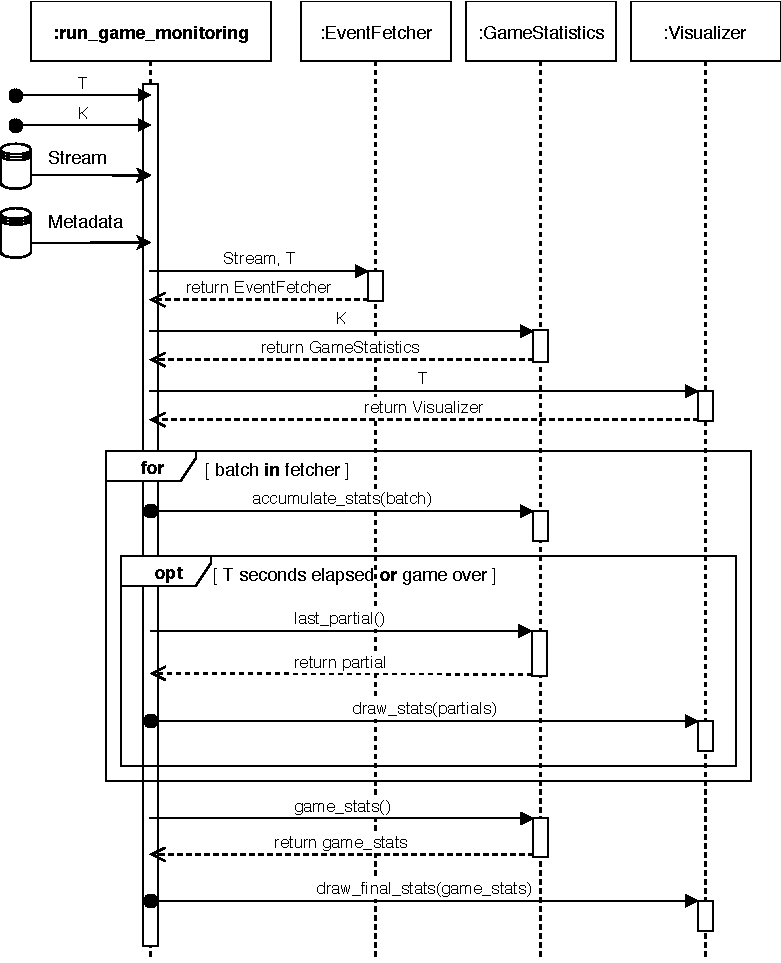
\includegraphics[height=.85\textheight]{UML/top_level_seq.pdf}
    \caption{Sequence diagram of the top-level interaction of main components.}
    \label{fig:top_level_seq}
\end{figure}
\begin{figure}[h]
    \centering
    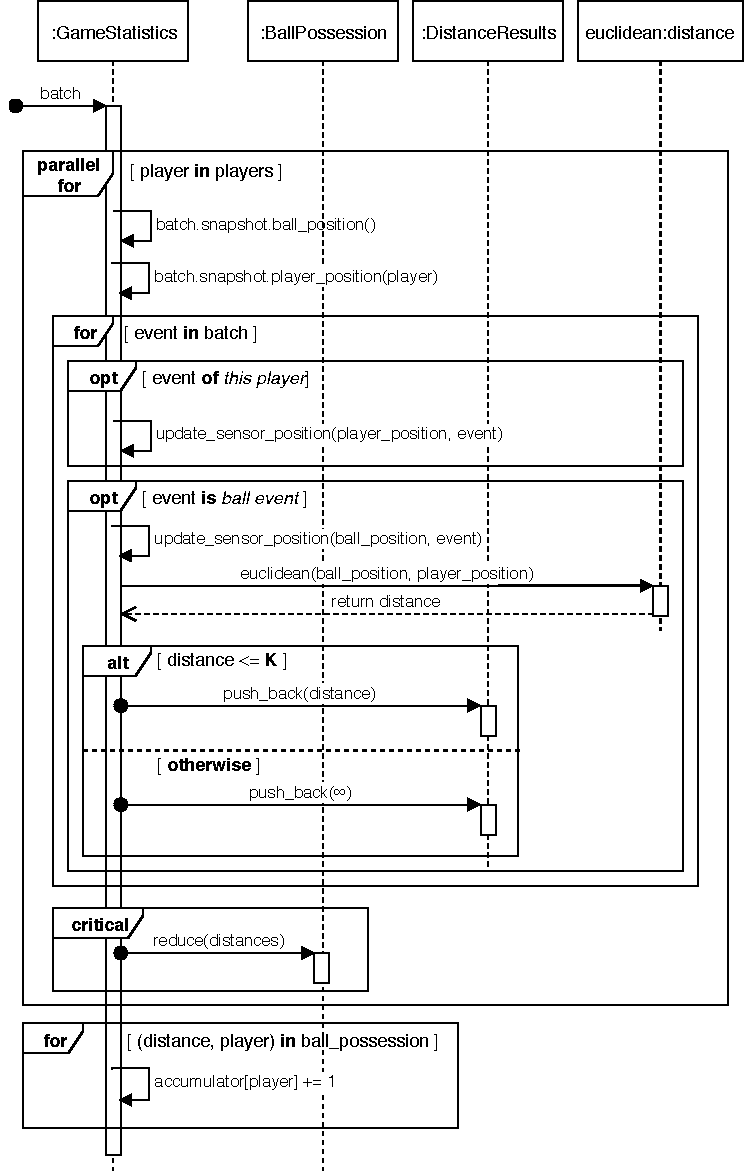
\includegraphics[height=.95\textheight]{UML/accumulate_stats.pdf}
    \caption{Sequence diagram of the process to compute ball possessions.}
    \label{fig:accumulate_stats_seq}
\end{figure}
\begin{figure}[h]
    \centering
    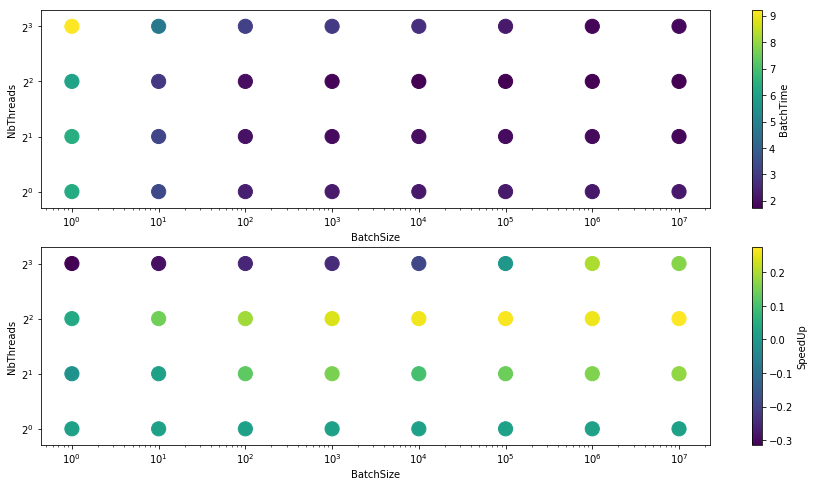
\includegraphics[width=1\textwidth]{Performance/speedup_analysis_7_1.png}
    \caption{On top, the application response time per-batch-processing with respect to the number of threads and the batch size. Below, the speed-up with respect to the single-threaded experiment.}
    \label{fig:perf1}
\end{figure}
\begin{figure}[h]
    \centering
    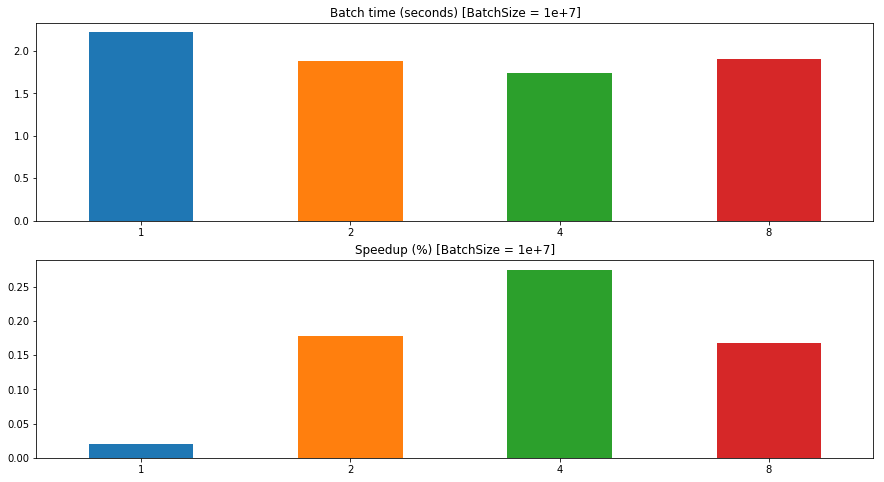
\includegraphics[width=1\textwidth]{Performance/speedup_analysis_12_1.png}
    \caption{On top, the application response time per-batch-processing with respect to the number of threads (fixed batch size). Below, the speed-ip with respect to the single-threaded experiment.}
    \label{fig:perf2}
\end{figure}

\end{document}
